\steppingstone{Every Length Needs a Name}
\label{stone:measuring}

The journey that led to PhiBase did not begin with numbers. It began with two triangles.

Imagine holding a golden triangle in your hand. Not a drawing, but a real one built from three straight pieces. Two of those pieces are the same length, while the third is shorter. Now make another triangle just like it. Join them together. Make another, and keep building.

Very quickly, something remarkable happens. No matter how many triangles you assemble, every straight edge in the construction is made from only two lengths. There are short pieces and long pieces, and no third length is needed.

Let the short length be

\[
1,
\]

and let the long length be

\[
\varphi=\frac{1+\sqrt{5}}{2}.
\]

A straight run containing seven short pieces and four long pieces has total length

\[
7+4\varphi.
\]

PhiBase records those two totals as

\[
P(7,4).
\]

The first coordinate counts the total number of short units embedded in the run. The second counts the total number of long units. The notation does not record the order in which the pieces appear. Many different arrangements can have the same PhiBase value.

For example, the sequences

\[
1,\;\varphi,\;\varphi,\;1,\;1
\]

and

\[
\varphi,\;1,\;1,\;1,\;\varphi
\]

both contain three short units and two long units. Both therefore have the same PhiBase value,

\[
P(3,2).
\]

They are different paths, but they have the same total embedded length.

\begin{figure}[htbp]
\centering
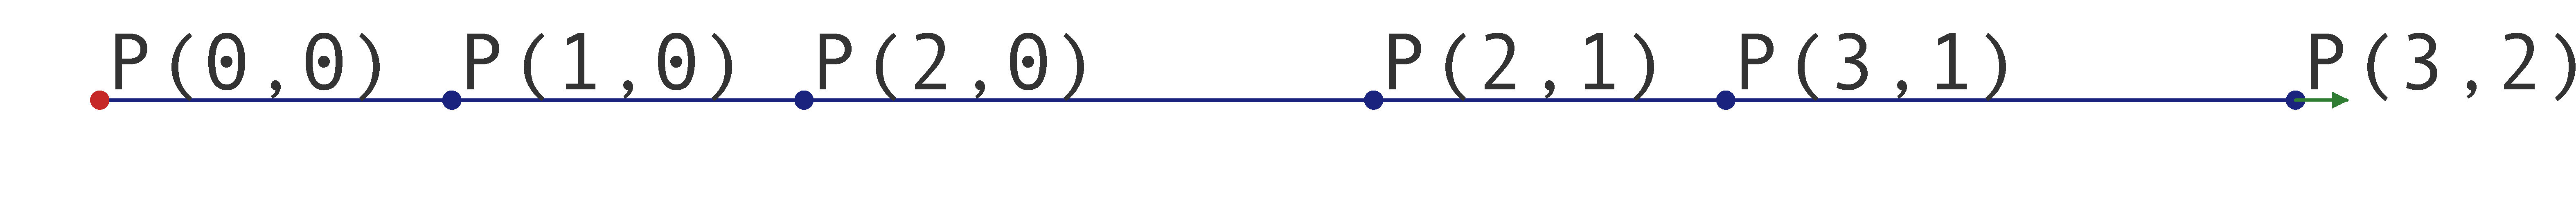
\includegraphics[width=.94\textwidth]{figures/turtle/line.pdf}
\caption{A straight sequence of short and long steps. Each marked point shows the accumulated PhiBase value of all steps before it.}
\label{fig:measuring-line}
\end{figure}

The marked points in Figure~\ref{fig:measuring-line} are cumulative totals. Each new short step adds

\[
P(1,0),
\]

and each new long step adds

\[
P(0,1).
\]

Thus

\[
P(0,0)=0
\]

means no length at all,

\[
P(1,0)=1
\]

means one short unit, and

\[
P(0,1)=\varphi
\]

means one long unit.

Nothing new has been invented. The value \(P(n,p)\) is simply the exact embedding

\[
n+p\varphi.
\]

Its usefulness is that the two kinds of length remain visible instead of being blurred into a decimal approximation.

\section*{Builder's Notebook}

Write the PhiBase value of each collection:

\[
\text{two short units},
\]

\[
\text{one short unit and one long unit},
\]

\[
\text{five long units},
\]

\[
\text{four short units and three long units},
\]

and

\[
\text{no units at all}.
\]

Then write two different arrangements that both have the value

\[
P(4,3).
\]

\section*{Looking Ahead}

PhiBase can name the total length of any straight collection of short and long units. The next question is what happens when two such totals are joined.
